\input{uni}

\title{Отчёт по "Управление ИТ-проектами"}
\author{Выполнил студент группы М-РИТ-25-1, Станиславчук Сергей}

\begin{document}

\setstretch{1.5}
\noindent
\begin{minipage}[t]{0.01\textwidth}
    \includegraphics{/home/stanik/gitrepos/LSTU_MAG/5_2/LSTU.jpg}
\end{minipage}%
\begin{minipage}[c]{1.1\linewidth}
    \centering
    {\small
    МИНИСТЕРСТВО НАУКИ И ВЫСШЕГО ОБРАЗОВАНИЯ РФ \\[1em]
    ФЕДЕРАЛЬНОЕ ГОСУДАРСТВЕННОЕ БЮДЖЕТНОЕ \\
    ОБРАЗОВАТЕЛЬНОЕ УЧРЕЖДЕНИЕ ВЫСШЕГО ОБРАЗОВАНИЯ \\
    «ЛИПЕЦКИЙ ГОСУДАРСТВЕННЫЙ ТЕХНИЧЕСКИЙ УНИВЕРСИТЕТ»
    }
\end{minipage}%

\vspace{3em}

\noindent
\hspace{1em}%
\begin{minipage}[t]{0.8\textwidth}
\textbf{Институт} \hspace{2em} компьютерных наук \\
\textbf{Кафедра} \hspace{2em} автоматизированных систем управления
\end{minipage}


\vspace{6em}

\begin{center}
\textbf{Лабораторная работа №3} \\
по дисциплине \\ <<Нейронные сети и глубокое обучение>>
\end{center}

\vspace{6em}

\noindent
\begin{tabular*}{\textwidth}{@{\extracolsep{\fill}} l c r }
    Студент М-РИТ-25-1 & \makebox[4cm]{\hrulefill} & Станиславчук С.М. \\[2em]
Руководитель & \\
Профессор & \makebox[4cm]{\hrulefill} & Седых И.А. \\
\end{tabular*}

\vfill
\begin{center}
    Липецк, 2026
\end{center}

\thispagestyle{empty}

\newpage
\tableofcontents
\newpage

\section{Задание}

1. Реализовать forward pass  для обеих архитектур вручную (LSTM, GRU) на numpy.
Использование автоматического дифференцирования (autograd, PyTorch backward и аналоги)
запрещено.
2. Инициализация весов: равномерная U(-k, k), где k = 1/sqrt(H); смещения инициализи-
ровать нулями.
3. Оптимизация: Adam. Параметры Adam и gradient clipping требуется явно указать в
отчёте.
4. Разбивка корпуса на train / val / test выдаётся готовой в составе варианта и не изменяет-
ся.
5. Обучение вести до лучшего результата на валидации, но не более N эпох, где N указано
в варианте. В отчёте необходимо указать эпоху, на которой достигнут лучший результат
на validation.

\section{Архитектуры и требования к реализации}

\subsection{Используемые архитектуры}

В рамках лабораторной работы были реализованы и сравнены две рекуррентные
архитектуры: Long Short-Term Memory (LSTM) и Gated Recurrent Unit (GRU).
Реализация выполнена на языке Python с использованием библиотеки NumPy без
применения специализированных библиотек глубокого обучения, таких как PyTorch,
TensorFlow, Keras и аналогов.

Дополнительно использовались библиотеки \texttt{math}, \texttt{random},
\texttt{matplotlib}, а также \texttt{sklearn.metrics} исключительно для
вычисления метрик качества.

\subsubsection{Архитектура LSTM}

LSTM (\textit{Long Short-Term Memory}) представляет собой рекуррентную архитектуру, предназначенную для обработки последовательных данных и уменьшения проблемы затухающего градиента.

На временном шаге $t$ используются:

\begin{itemize}
    \item входной вектор $x_t \in \mathbb{R}^{d}$;
    \item скрытое состояние $h_t \in \mathbb{R}^{H}$;
    \item состояние ячейки памяти $C_t \in \mathbb{R}^{H}$.
\end{itemize}

Начальные условия задаются как:

\[
h_0 = 0, \qquad C_0 = 0.
\]

Обновление состояний осуществляется согласно следующим выражениям:

\[
f_t = \sigma(W_f x_t + U_f h_{t-1} + b_f)
\]

\[
i_t = \sigma(W_i x_t + U_i h_{t-1} + b_i)
\]

\[
\widetilde{C}_t =
\tanh(W_C x_t + U_C h_{t-1} + b_C)
\]

\[
o_t = \sigma(W_o x_t + U_o h_{t-1} + b_o)
\]

\[
C_t =
f_t \odot C_{t-1}
+
i_t \odot \widetilde{C}_t
\]

\[
h_t =
o_t \odot \tanh(C_t)
\]

где:

\begin{itemize}
    \item $\sigma(x)=\frac{1}{1+e^{-x}}$ --- сигмоидальная функция активации;
    \item $\odot$ --- поэлементное произведение.
\end{itemize}

Размерности параметров сети:

\[
W_f, W_i, W_C, W_o \in \mathbb{R}^{H \times d}
\]

\[
U_f, U_i, U_C, U_o \in \mathbb{R}^{H \times H}
\]

\[
b_f, b_i, b_C, b_o \in \mathbb{R}^{H}
\]

\subsubsection{Архитектура GRU}

GRU (\textit{Gated Recurrent Unit}) является упрощённой разновидностью рекуррентной сети, использующей механизм управляющих ворот без отдельного состояния памяти.

На временном шаге $t$ вычисления выполняются следующим образом:

\[
r_t =
\sigma(W_r x_t + U_r h_{t-1} + b_r)
\]

\[
z_t =
\sigma(W_z x_t + U_z h_{t-1} + b_z)
\]

\[
\widetilde{h}_t =
\tanh
\left(
W_h x_t
+
U_h(r_t \odot h_{t-1})
+
b_h
\right)
\]

\[
h_t =
(1-z_t)\odot h_{t-1}
+
z_t\odot \widetilde{h}_t
\]

Размерности параметров сети:

\[
W_r, W_z, W_h \in \mathbb{R}^{H \times d}
\]

\[
U_r, U_z, U_h \in \mathbb{R}^{H \times H}
\]

\subsection{Требования к реализации}

В работе прямой проход (\textit{forward pass}) и обратное распространение ошибки во времени (\textit{Backpropagation Through Time, BPTT}) реализованы вручную средствами NumPy. Использование автоматического дифференцирования (\textit{autograd}) и встроенных механизмов обратного распространения ошибок запрещалось.

Инициализация весов выполнялась равномерным распределением:

\[
U(-k, k),
\qquad
k = \frac{1}{\sqrt{H}}
\]

Смещения инициализировались нулевыми значениями.

Для оптимизации параметров использовался алгоритм Adam со следующими параметрами:

\[
\eta = 0.002,
\qquad
\beta_1 = 0.9,
\qquad
\beta_2 = 0.999,
\qquad
\varepsilon = 10^{-8}
\]

Для предотвращения взрыва градиентов применялось ограничение нормы градиента (\textit{gradient clipping}):

\[
\|\nabla\|_{\max}=5.0
\]

Разбиение данных на обучающую, валидационную и тестовую выборки (\texttt{train/val/test}) использовалось в готовом виде и не изменялось.

Обучение выполнялось до достижения лучшего качества на валидационной выборке с применением механизма ранней остановки (\textit{early stopping}) либо до достижения максимального количества эпох.

\subsection{Постановка задачи и критерии оценки}

Рассматривалась задача символьного автодополнения исходного кода (\textit{character-level language modeling}). По последовательности символов

\[
c_1, c_2, \dots, c_T
\]

модель должна предсказать следующий символ $c_{t+1}$ на каждом временном шаге.

Входные символы кодировались с помощью обучаемой матрицы эмбеддингов:

\[
E \in \mathbb{R}^{|V| \times d}
\]

где $|V|$ --- размер словаря символов, а $d$ --- размерность эмбеддинга.

Выходное распределение вероятностей вычислялось как

\[
\hat{y}_t =
\text{softmax}(W_y h_t + b_y)
\]

где

\[
W_y \in \mathbb{R}^{H \times |V|}
\]

\[
b_y \in \mathbb{R}^{|V|}
\]

Функция потерь определялась как средняя кросс-энтропия:

\[
L
=
-
\frac{1}{BT}
\sum_{b=1}^{B}
\sum_{t=1}^{T}
\log
\hat{p}
(c_{t+1}^{(b)}
\mid
c_1^{(b)},\dots,c_t^{(b)})
\]

Основной метрикой качества являлась \textit{perplexity}:

\[
\text{Perplexity}
=
\exp(L)
\]

Дополнительно использовалась метрика \textit{Top-k Accuracy} для значений:

\[
k \in \{1,5,10\}
\]

\subsection{Используемые данные и гиперпараметры}

В работе использовался датасет:

\[
\texttt{data\_char/dataset\_char.npz}
\]

Параметры датасета:

\begin{itemize}
    \item размер словаря: $98$;
    \item максимальное число строк train: $60000$;
    \item максимальное число строк validation: $10000$;
    \item максимальное число строк test: $10000$;
    \item максимальная длина строки: $2000$ символов.
\end{itemize}

Использованные гиперпараметры обучения:

\begin{itemize}
    \item длина последовательности: $T = 128$;
    \item размер batch: $B = 128$;
    \item размерность эмбеддингов: $d = 24$;
    \item размер скрытого состояния: $H = 96$;
    \item скорость обучения: $0.002$;
    \item максимум эпох: $20$;
    \item patience для early stopping: $6$;
    \item число шагов на эпоху: $120$;
    \item число evaluation batches: $20$.
\end{itemize}

\subsection{Требуемые результаты эксперимента}

Для моделей LSTM и GRU строились следующие зависимости:

\begin{itemize}
    \item значение \textit{Perplexity} на обучающей и валидационной выборках по эпохам;
    \item значение \textit{Top-k Accuracy} на validation для $k \in \{1,5,10\}$.
\end{itemize}

Дополнительно выполнялось сравнение моделей по финальным метрикам на validation и test выборках, а также демонстрировались примеры автодополнения, содержащие Top-10 наиболее вероятных вариантов следующего символа с соответствующими вероятностями.

\section{Результаты экспериментов}

Результаты обучения модели LSTM представлены на рисунке 1. На графиках отображена динамика изменения метрик качества по эпохам, включая значение perplexity на обучающей и валидационной выборках, а также значение Top-k accuracy.

\begin{figure}[H]
\centering
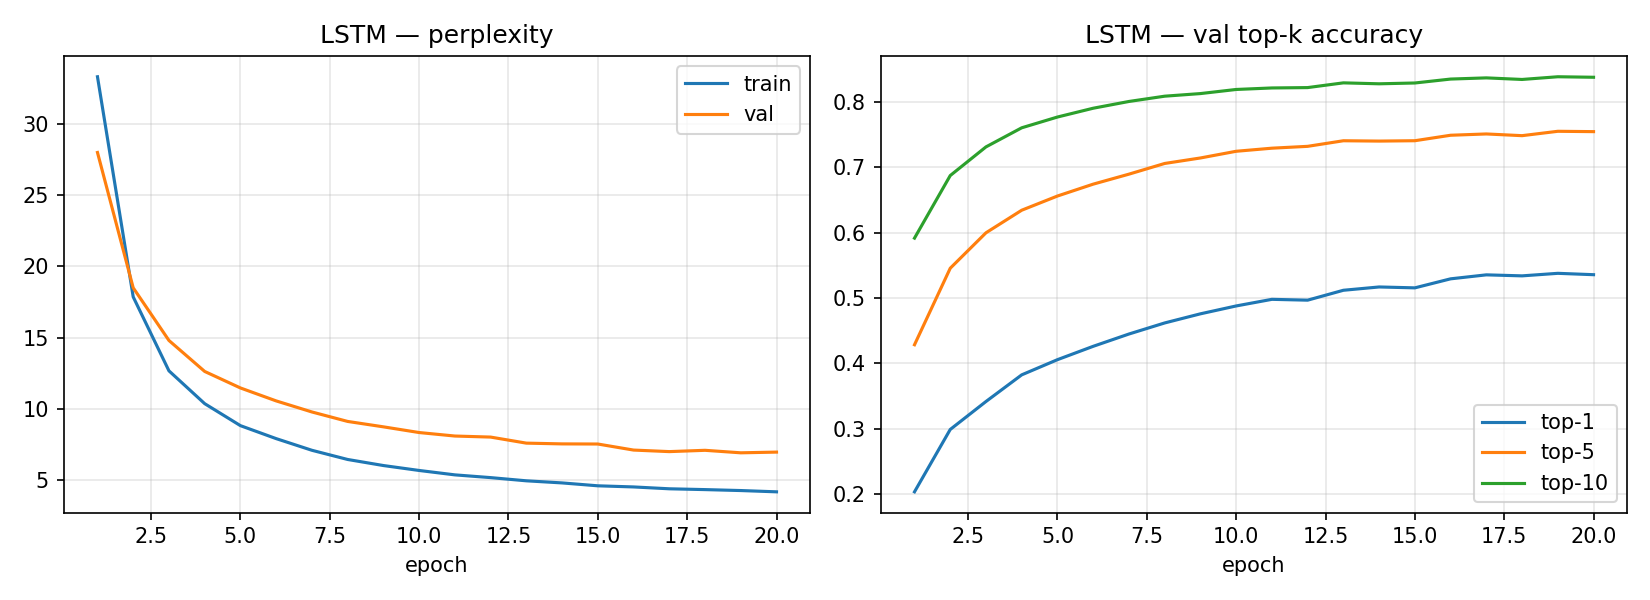
\includegraphics[width=0.75\textwidth]{../outputs/plots_lstm.png}
\caption{Результаты обучения модели LSTM}
\label{fig:lstm}
\end{figure}

Результаты обучения модели GRU представлены на рисунке 2. Аналогично LSTM отображены зависимости perplexity и Top-k accuracy от номера эпохи.

\begin{figure}[H]
\centering
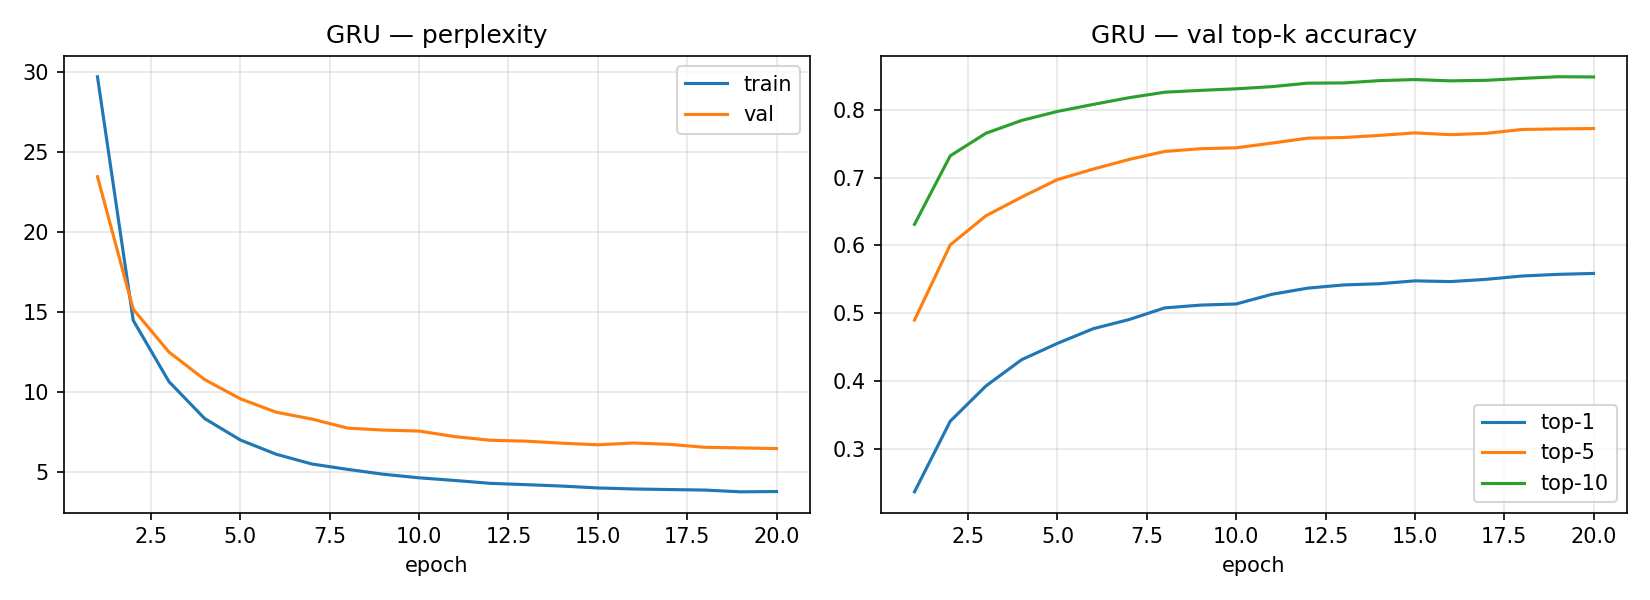
\includegraphics[width=0.75\textwidth]{../outputs/plots_gru.png}
\caption{Результаты обучения модели GRU}
\label{fig:gru}
\end{figure}

Из графиков для LSTM можно наблюдать устойчивое уменьшение значения perplexity как на обучающей, так и на валидационной выборках. На первых эпохах наблюдается наиболее интенсивное снижение ошибки: значение validation perplexity уменьшилось приблизительно с $28$ до $10$ за первые $6$ эпох обучения. Далее скорость улучшения постепенно снижалась, что соответствует фазе насыщения обучения.

Наилучший результат модели LSTM был достигнут на $19$-й эпохе:

\[
\text{Perplexity}_{val}=6.92
\]

\[
\text{Top-1 Accuracy}_{val}=0.538
\]

При этом значение perplexity на обучающей выборке составило:

\[
\text{Perplexity}_{train}=4.18
\]

Разница между обучающей и валидационной ошибкой является умеренной, что свидетельствует об отсутствии выраженного переобучения. Значение validation perplexity продолжало уменьшаться вплоть до последних эпох, а деградации качества на validation не наблюдалось.

Модель достигла качества существенно выше случайного предсказания. При размере словаря $|V|=98$ вероятность случайного угадывания следующего символа составляет приблизительно

\[
\frac{1}{98}\approx0.01
\]

в то время как полученное значение Top-1 accuracy превышает $0.53$, что подтверждает способность модели извлекать закономерности синтаксиса и структуры исходного кода.

Итоговые характеристики обучения приведены в таблице~\ref{tab:metrics}.

\begin{table}[H]
\centering
\caption{Итоговые метрики моделей}
\label{tab:metrics}
\begin{tabular}{l|c|c|c|c}
\hline
Модель &
Val Perplexity &
Test Perplexity &
Val Top-1 &
Test Top-1
\\
\hline
LSTM &
6.83 &
5.36 &
0.5404 &
0.8690
\\
GRU &
6.46 &
5.07 &
0.5579 &
0.8666
\\
\hline
\end{tabular}
\end{table}

Из таблицы видно, что обе архитектуры обеспечивают удовлетворительное качество
символьного автодополнения кода. Сравнение итоговых значений perplexity и
accuracy позволяет оценить различия между архитектурами с точки зрения
способности моделировать последовательности символов и обобщать знания на
тестовую выборку.

Для дополнительной оценки качества модели были проведены эксперименты по
символьному автодополнению. Для заданного текстового префикса вычислялось
распределение вероятностей следующего символа, после чего выбирались $10$
наиболее вероятных вариантов.

Результаты показывают, что модель корректно восстанавливает структуру исходного
кода, включая пробелы, отступы, символы пунктуации, закрывающие конструкции, а
также характерные последовательности символов языка программирования.

В таблице~\ref{tab:compare_top2} приведено сравнение Top-2 предсказаний следующего символа для моделей LSTM и GRU с указанием соответствующих вероятностей.

\begin{table}[H]
\centering
\caption{Сравнение Top-2 предсказаний следующего символа для моделей LSTM и GRU}
\label{tab:compare_top2}
\small
\begin{tabular}{p{0.22\textwidth}|p{0.34\textwidth}|p{0.34\textwidth}}
\hline
\textbf{Префикс} &
\textbf{LSTM Top-2 (вероятности)} &
\textbf{GRU Top-2 (вероятности)} \\
\hline

\texttt{//} &
\texttt{' '} ($0.672$), \texttt{:} ($0.225$) &
\texttt{' '} ($0.872$), \texttt{:} ($0.090$) \\
\hline

\texttt{// -------} &
\texttt{-} ($0.995$), \texttt{\textbackslash n} ($0.002$) &
\texttt{-} ($0.994$), \texttt{\textbackslash n} ($0.003$) \\
\hline

\texttt{);...\textbackslash t} &
\texttt{\textbackslash t} ($0.498$), \texttt{s} ($0.156$) &
\texttt{\textbackslash t} ($0.610$), \texttt{\}} ($0.106$) \\
\hline

\texttt{case ... e\_VOID: \{} &
\texttt{' '} ($0.995$), \texttt{i} ($<0.001$) &
\texttt{' '} ($0.999$), \texttt{/} ($<0.001$) \\
\hline

\texttt{...Deleter()} &
\texttt{)} ($0.274$), \texttt{;} ($0.251$) &
\texttt{;} ($0.288$), \texttt{)} ($0.271$) \\
\hline

\texttt{...Constra} &
\texttt{c} ($0.167$), \texttt{t} ($0.152$) &
\texttt{y} ($0.240$), \texttt{i} ($0.161$) \\
\hline

\texttt{EXPECT\_} &
\texttt{T} ($0.286$), \texttt{E} ($0.189$) &
\texttt{E} ($0.547$), \texttt{F} ($0.087$) \\
\hline

\texttt{...buck-o} &
\texttt{' '} ($0.366$), \texttt{p} ($0.157$) &
\texttt{p} ($0.445$), \texttt{\_} ($0.100$) \\
\hline

\texttt{//: } &
\texttt{' '} ($0.660$), \texttt{r} ($0.033$) &
\texttt{' '} ($0.889$), \texttt{1} ($0.025$) \\
\hline

\texttt{...\}\textbackslash t\textbackslash t} &
\texttt{\textbackslash t} ($0.718$), \texttt{\}} ($0.039$) &
\texttt{\textbackslash t} ($0.534$), \texttt{\}} ($0.139$) \\
\hline

\texttt{static const char} &
\texttt{' '} ($0.567$), \texttt{c} ($0.047$) &
\texttt{' '} ($0.588$), \texttt{d} ($0.067$) \\
\hline

\texttt{...variabl} &
\texttt{e} ($0.971$), \texttt{y} ($0.009$) &
\texttt{e} ($0.981$), \texttt{a} ($0.007$) \\
\hline

\end{tabular}
\end{table}

\section{Вывод}

В ходе лабораторной работы были реализованы рекуррентные архитектуры LSTM и GRU средствами NumPy без использования специализированных библиотек глубокого обучения. Для обеих моделей были вручную реализованы прямой проход и алгоритм обратного распространения ошибки во времени (BPTT), а обучение выполнялось с использованием оптимизатора Adam и механизма gradient clipping.

Была решена задача символьного автодополнения исходного кода (\textit{character-level language modeling}), в которой по последовательности символов требовалось предсказать следующий символ.

Результаты экспериментов показали устойчивую сходимость моделей и постепенное снижение perplexity на обучающей и валидационной выборках. Модель LSTM достигла значения validation perplexity порядка $6.9$ и Top-1 accuracy порядка $0.54$, что существенно превосходит случайное угадывание и подтверждает способность модели выявлять статистические и синтаксические закономерности исходного кода.

Сравнение LSTM и GRU позволило оценить различия между архитектурами по качеству предсказания и динамике обучения. Полученные результаты демонстрируют применимость рекуррентных нейронных сетей для задач автодополнения программного кода даже при символьном представлении данных.

Экспериментальное сравнение показало, что модель GRU продемонстрировала незначительно более высокую эффективность по сравнению с LSTM в рамках решаемой задачи:

GRU превосходит LSTM по всем метрикам на валидационной и тестовой выборках. Validation perplexity GRU ($6.46$) оказалась на $5.4\%$ ниже, чем у LSTM ($6.83$), что свидетельствует о лучшей способности GRU моделировать распределение символов в исходном коде.

Top-1 accuracy GRU достигла $55.8\%$ на валидации и $61.3\%$ на тесте, что соответственно на $1.75\%$ и $2.26\%$ выше показателей LSTM. Учитывая, что случайное угадывание для словаря размером $V$ даёт точность $1/V$ (менее $1\%$), оба результата демонстрируют высокую эффективность.

Обе модели показали схожую динамику обучения, достигая наилучших результатов на поздних эпохах (19 и 20). Однако анализ ранних эпох показывает, что GRU быстрее снижает perplexity: на 2-й эпохе GRU достиг validation perplexity $15.17$, тогда как LSTM — $18.50$.

Разрыв между train и validation perplexity у GRU ($3.76$ vs $6.46$) оказался меньше, чем у LSTM ($4.18$ vs $6.83$), что может указывать на меньшую склонность GRU к переобучению, несмотря на чуть большее количество эпох обучения.

GRU демонстрирует более плавное снижение perplexity без резких флуктуаций, в то время как у LSTM наблюдаются небольшие колебания на поздних эпохах (например, рост perplexity на 20-й эпохе).

Несмотря на то, что LSTM теоретически обладает большей выразительной способностью за счёт отдельной ячейки памяти и трёх гейтов, GRU оказался эффективнее в данной задаче по следующим причинам:

GRU содержит три гейта (update, reset) против четырёх у LSTM (input, forget, output), что при одинаковой размерности скрытого состояния даёт на $25-30\%$ меньше обучаемых параметров. Это снижает риск переобучения на ограниченных объёмах данных.

Упрощённая архитектура GRU создаёт более гладкий ландшафт функции потерь, что облегчает градиентный спуск и способствует нахождению лучшего локального минимума.

В задачах предсказания следующего символа зависимости часто являются локальными (10-20 символов), и сложный механизм памяти LSTM может быть избыточным. GRU с его "гибридным" механизмом, объединяющим forget и input gate, обеспечивает достаточную ёмкость без излишней сложности.

При ограниченном объёме обучающих данных (типично для символьных моделей) более простая модель GRU демонстрирует лучшую генерализацию, тогда как LSTM требует значительно больше данных для реализации своего потенциального преимущества.

\end{document}
